\renewcommand{\BrainFuckChapter}{
  {+}{+}{+}{+}{[}{+}{+}{+}{+}{>}{-}{-}{-}{<}{]}{>}{.}{+}{[}{-}{-}{-}{>}{+}{<}{]}{>}{+}{+}{+}{.}{-}{.}{-}{-}{-}{-}{-}{-}{-}{-}{-}{-}{-}{.}{+}{+}{+}{+}{+}{+}{+}{+}{+}{.}{+}{+}{+}{+}{+}{+}{+}{+}{+}{.}{-}{-}{.}{-}{-}
  {-}{-}{-}{-}{-}{-}{-}{-}{.}{+}{+}{+}{+}{+}{+}{.}{-}{.}{+}{+}{+}{+}{+}{.}{>}{>}{<}{>}{+}{<}{-}{<}{<}{-}{-}{-}{>}{<}{<}{-}{>}{<}{>}{>}{>}{>}{-}{<}{<}{>}{+}{-}{<}{+}{>}{<}{-}{>}{<}{>}{-}{<}{+}{-}{<}{<}{>}{+}{-}{+}
}
\renewcommand{\LifeChapter}{y}

\chapter{Conclusions}
In this section we draw conclusions about the work developed in the
scope of this thesis.
%

This chapter is divided as follows.
%
First, we answer the research questions introduced in
\Cref{sec:intro:research-goals}.
%
Second, we list the contributions that resulted from the developed
work.
%
Finally, we discuss possible paths of future research.


\section{Research Questions}

\begin{description}[leftmargin=!,labelwidth=\widthof{\bfseries \Cref{rq:optimizations} ---}]
\item [\Cref{rq:optimizations} ---] Is it possible to optimize
  \staccato{} to minimize redundant/superfluous computations?
\end{description}

We found that the \staccato{} algorithm could be improved to achieve
a higher computational efficiency.
%
To this end we proposed $3$ optimizations.
%
The first optimization prevents multiple examinations of the same set.
%
The second optimization preemptively filters elements guaranteed not
to form \acp{MHS}.
%
The third optimization prevents the examination of search tree
branches guaranteed not to yield any \acp{MHS}.

The conducted benchmarks showed that the proposed optimizations
resulted, on average, in a $34000\times$ performance improvement for
small problems and in a $186\times$ improvement for large problems.

\begin{description}[leftmargin=!,labelwidth=\widthof{\bfseries \Cref{rq:optimizations} ---}]
\item [\Cref{rq:scalability} ---] Is it possible to parallelize
  \staccato{} as way of reducing the diagnostic latency?
\end{description}

The \staccato{} algorithm can be successfully parallelized.
%
To achieve this goal, we proposed a Map-Reduce parallelization of
\staccato{}.
%
The parallel algorithm makes use of a pseudo-random generator to
evenly distribute the computations among threads without needing any
communication apart from the initial seed sharing.

The conducted benchmarks showed that the proposed parallelization
approach scales with minimal overheads: the algorithm exhibits a
similar throughput per thread in both small/large problems and
sequential/parallel setups.
%

\begin{description}[leftmargin=!,labelwidth=\widthof{\bfseries \Cref{rq:optimizations} ---}]
\item [\Cref{rq:fuzzy-error-encoding} ---] How to encode fuzzy error
  symptoms?
\end{description}

We proposed a fuzzy logic generalization over the classical binary
error representation.
%
Instead of classifying transactions in terms of pass/fail, we suggest
the usage of set membership functions ($\ferror[x]$).
%
Such functions map an arbitrary input onto the interval $[0,1]$,
enabling the representation of $3$ types of transaction outcomes:
correct ($\ferror = 0$), incorrect ($\ferror = 1$) and degraded ($0 <
\ferror < 1$).

A consequence of the new error model is that a degraded transaction
exhibits both correct and incorrect behaviors simultaneously, however
with different degrees.
%
This is due to the fact that the pass and fail sets are complimentary
and, therefore, the sum of both set membership functions must be equal
to $1$ (\ie, $\ferror[P](x) = 1 - \ferror(x)$).

\begin{description}[leftmargin=!,labelwidth=\widthof{\bfseries \Cref{rq:optimizations} ---}]
\item [\Cref{rq:SFL-fuzzy-error-generalization} ---] How to improve
  \ac{SFL} to make use of the fuzzy error information?
\end{description}

To use the fuzzy error information we improve the \ac{SFL} framework
by making use of the concept of probability of a fuzzy event, which is
defined as:
\begin{equation}
  \pr{\alpha} = \sum_{x\in\Omega}{\ferror[x](\alpha) \cdot \pr{x}}
\end{equation}
\noindent
where $\Omega$ is the set of possible outcomes which, in the case of error
diagnosis, is equal to $\set{P,F}$.

Applying the above formula to the \ac{SFL} framework results in the
following generalization:

\begin{equation}
  \posterior{}   =  \pr{d} \times
  \frac{
    \displaystyle \prod_{i \in 1..N}
    \overbrace{\vphantom{\big(}e_i}^{\ferror(\alpha)} \cdot
    \overbrace{\vphantom{\big(}\big(1 - \gFunc{}\big)}^{\pr{x=F \mid A,d}} +
    \overbrace{\vphantom{\big(}(1-e_i)}^{\ferror[P](\alpha)} \cdot
    \overbrace{\vphantom{\big(}\gFunc{}}^{\pr{x=P \mid A,d}}}
  {\pr{A, e}}
\end{equation}
\noindent
The classical \ac{SFL} approach
(\CrefPageSee{eq:intro:likelihood-func}) is a special case of the
proposed generalization when $\forall_{e_i} : e_i \in \set{0,1}$.

The conducted benchmarks showed that, for our setup, the fuzzy
approach improved the diagnostic quality in $65\%$ of the test cases
and performed at least as good as the classical approach in $94\%$ of
the test cases.
%
Furthermore, the fuzzy diagnostic was, on average, $20\%$ more
accurate than classical approach.

\begin{description}[leftmargin=!,labelwidth=\widthof{\bfseries \Cref{rq:optimizations} ---}]
\item [\Cref{rq:feedback} ---] How to enable \ac{SFL} to adapt to
  different systems based on previous diagnostic experience?
\end{description}

To enable \ac{SFL} to make use of previous diagnostic experience, we
proposed an improved goodness modeling approach.
%
To this end, we introduced the concept of a feedback loop in \ac{SFL},
consisting of a pass ($\FB_{0j}$) and a fail ($\FB_{1j}$) observation
lists for each component $j$.
%
Each list is defined as:
\begin{equation}
  \FB_{ej} = \angledlist{\ST_1, ...,  \ST_k, ..., \ST_K}
\end{equation}
\noindent
where $\ST$ represents a set of system variables' values in which
component $j$ was observed to perform either nominally or erroneously.

Each list is then used to create a \ac{KDE} as follows:
\begin{equation}
  \KDE = \frac {1}{\BW}{\mathlarger{\sum_{\ST^\prime \in \FB_{ej}}} \fn{K}\bigg(\frac{\ST - \ST^\prime}{\BW}\bigg)}
\end{equation}

Intuitively, the \ac{KDE} works like a continuous histogram,
estimating how the pass/fail states are spread across the entire state
space.

The final modeling step consist of using both the pass and fail \acp{KDE}
to estimate the component's goodness.
%
Formally, the improved goodness model is defined as:
\begin{equation}
  \supergj = \frac{\KDE[0j]}{\KDE[0j] + \KDE[1j]}
\end{equation}


\begin{description}[leftmargin=!,labelwidth=\widthof{\bfseries \Cref{rq:optimizations} ---}]
\item [\Cref{rq:system-state} ---] How to incorporate information
  about the system's state in \ac{SFL}?
\end{description}

To make use of the system state in the diagnostic process, we
generalized the spectrum's activity matrix as:
\begin{equation}
  A_{ij} = \begin{cases}
    \clubsuit, & \textrm{if $c_j$ does not have a $\supergj{}$ model and was involved in transaction $i$} \\
    \angledlist{st_{1}, \cdots, st_{k}}, & \textrm{if $c_j$ has a $\supergj{}$ model and was involved in transaction $i$}\\
    \emptyset, & \textrm{otherwise}
  \end{cases}
\end{equation}
\noindent
The improved spectrum enables the capture of the system's state which,
in turn, is plugged onto the improved goodness models.
%

To incorporate the improved spectrum and goodness models onto the
\ac{SFL} framework, we define the generalize the transaction goodness
function as:
\begin{equation}
  \displaystyle \gFunc = \prod_{j \in (d \cap A_i)}
  \begin{cases}
    g_j, & \textrm{if} A_{ij} = \clubsuit\\
    (1-\alpha_j) \cdot g_j + \alpha_j \cdot \supergFunc[j,A_{ij}], & \textrm{otherwise}
  \end{cases}
\end{equation}
\begin{equation}
  \supergFunc = \prod_{st \in S} \supergj{}
\end{equation}
\noindent
where $\alpha_j \in [0,1]$ is a model confidence parameter.
%
This parameter enables the \ac{SFL} framework to fallback to the
\ac{MLE} goodness model as the state-aware goodness model gradually
becomes obsolete.
%
In fact, the classical \ac{SFL} approach
(\CrefPageSee{eq:intro:g-func}) is a special case of the proposed
generalization when $\forall_{\alpha_j} : \alpha_j = 0$.


\section{Contributions}
\label{sec:conclusions:contributions}
Overall, the work developed for this thesis resulted in $3$
main contributions:
\begin{enumerate}
\item We developed a \ac{SFL} candidate generation algorithm that is
  both more efficient than the state-of-the-art algorithm
  (\CrefPageSee[]{sec:mhs2o:approach}) and can make use of multiple
  \acp{CPU} to compute diagnostic candidates
  (\CrefPageSee[]{sec:mhs2p:approach}).
  %
  Furthermore, we released a reference implementation under the GNU
  Lesser General Public
  License\footnote{\url{https://www.gnu.org/licenses/lgpl.html}},
  available at \mhsIIURL{}.

\item We proposed a fuzzy logic-based approach to error detection
  enabling a more accurate representation of performance degradation
  errors
  (\CrefPageSee[]{sec:fuzzinel:approach:fuzzy-error-detection}).
  %
  Furthermore, we improved the spectrum-based reasoning framework for
  fault localization to incorporate the improved error representation
  (\CrefPageSee[]{sec:fuzzinel:approach:fuzzy-error-diagnosis}).

\item We proposed a \ac{KDE}-based approach to model the components'
  goodnesses as a function of the system state
  (\CrefPageSee[]{sec:nfge:approach:modeling}).
  %
  Furthermore, we improved the spectrum-based reasoning framework for
  fault localization to incorporate the improved goodness estimation
  (\CrefPageSee[]{sec:nfge:approach:ranking}).
\end{enumerate}

In addition to the main contributions, in the scope of this thesis:
\begin{itemize}
\item We introduced the state spectrum data structure, which generalizes
  over a set of existent types of spectra (\eg, hit spectrum, count
  spectrum, \etc) and enables a more precise abstraction of the
  system's executions.
\item We introduced the concept of a feedback loop in the scope of
  \ac{SFL}.
\end{itemize}

\section{Future Work}
In this section we discuss future research topics related to the
material presented in this thesis.


\subsection{Goodness Modeling}
\subsubsection*{Feedback Generation}

Given a set of state spectra and their respective correct diagnostic
candidates, it should be possible to automatically extract information
to generate the feedback spectra.
%
To illustrate how this could be accomplished in practice, consider the
state spectrum in \Cref{fig:conclusions:state-spectrum} for which the
correct diagnostic candidate was determined to be $d = \set{1,2}$.
%

\begin{figure}[!ht]
  \begin{tabular}[b]{c|ccc|c}
    \multirow{2}{*}{$i$} & \multicolumn{3}{c|}{$A$}                             & \multirow{2}{*}{$e$}                   \\
    \cline{2-4}
                         & $c_1$                                                & $c_2$                 & $\cdots$ &     \\ \hline
    $1$                  & \cellcolor{clra}   $\angledlist{0.42}$      & $\emptyset$           & $\cdots$ & $0$ \\
    $2$                  & \cellcolor{clra}   $\angledlist{0.86,1.86}$ & $\emptyset$           & $\cdots$ & $0$ \\
    $3$                  & \cellcolor{clra}   $\angledlist{0.14}$      & $\angledlist{\cdots}$ & $\cdots$ & $0$ \\
    $4$                  & \cellcolor{clra}   $\angledlist{0.58,1.46}$ & $\angledlist{\cdots}$ & $\cdots$ & $0$ \\
    $5$                  & \cellcolor{clrb} $\angledlist{1.05}$      & $\emptyset$           & $\cdots$ & $1$ \\
    $6$                  & \cellcolor{clrb} $\angledlist{1.35}$      & $\emptyset$           & $\cdots$ & $1$ \\
    $7$                  & \cellcolor{clrb} $\angledlist{1.79}$      & $\emptyset$           & $\cdots$ & $1$ \\
    $8$                  & \cellcolor{clrc}   $\angledlist{0.49,1.34}$ & $\emptyset$           & $\cdots$ & $1$ \\
    $9$                  & \cellcolor{clrc}   $\angledlist{1.67}$      & $\angledlist{\cdots}$ & $\cdots$ & $1$ \\
    $10$                 & \cellcolor{clrc}   $\angledlist{0.49,0.81}$ & $\angledlist{\cdots}$ & $\cdots$ & $1$ \\
  \end{tabular}
  \caption{State spectrum}
  \label{fig:conclusions:state-spectrum}
\end{figure}

Analyzing the spectrum, we can see that the states of the transactions
in which $c_1$ was activated can be divided into $3$ categories:
nominal, error, and undetermined.
%
The categorization is a function of $3$ factors: the number of
activations of the target component, the number of activated faulty
components, and the outcome of the transaction
(\Cref{fig:conclusions:state-categorization}).

\begin{figure}[!ht]
  \renewcommand{\arraystretch}{1.2}
  \newcolumntype{x}{C{3em}}
  \begin{tabular}{ccc|c}
    Component States & Faulty Components & Transaction Outcome &                                        \\\hline
    One              & One               & Pass                & \cellcolor{clra} Nominal      \\
    More than one    & One               & Pass                & \cellcolor{clra} Nominal      \\
    One              & More than one     & Pass                & \cellcolor{clra} Nominal      \\
    More than one    & More than one     & Pass                & \cellcolor{clra} Nominal      \\
    One              & One               & Fail                & \cellcolor{clrb} Error      \\
    More than one    & One               & Fail                & \cellcolor{clrc} Undetermined \\
    One              & More than one     & Fail                & \cellcolor{clrc} Undetermined \\
    More than one    & More than one     & Fail                & \cellcolor{clrc} Undetermined \\

  \end{tabular}
  \caption{State categorization}
  \label{fig:conclusions:state-categorization}
\end{figure}

The nominal and error states can be directly added to the feedback
spectrum whereas, the undetermined states cannot.
%
The simplest approach for handling undetermined states is to simply
ignore them.
%
The major drawback of this approach is that the available information
is not used to its full extent.

A more convoluted approach is to make use of a clustering algorithm
such as \ac{KNN} \citep{Altman92}.
%
In short, \ac{KNN} classifies a point based on the most frequent class
among its $K$ nearest (classified) neighbors.
%
\Cref{fig:conclusions:knn} illustrates how the undetermined states in
\Cref{fig:conclusions:state-spectrum} would be classified by \ac{KNN}
with $K=3$.
%
It is worth to note that all undetermined states should be
reclassified every time new diagnosed state spectra is available for
feedback extraction.

\begin{figure}[!ht]
  \includegraphics[page=6]{figures/conclusions/figures/main.pdf}
  \caption{\acs{KNN}-based feedback spectrum extraction example}
  \label{fig:conclusions:knn}
\end{figure}

Another possible approach is to still use the \ac{KNN} algorithm but,
instead of all states having equal weight in the goodness calculation,
they may have different weights.
%
To this end, we generalize \Cref{eq:nfge:feedback-spectrum} as:
\begin{equation}
  \label{eq:conclusions:feedback-spectrum}
  \FB_{ej} = \angledlist{(\ST_1, w_1), ...,  (\ST_k, w_k), ..., (\ST_K,w_K)}
\end{equation}
\noindent
where $w_k$ represents the weight of observation $\ST_k$.
%
To account for this generalization, we redefine
\Cref{eq:nfge:kde} as:
\begin{equation}
  \KDE = \frac {1}{bw}{\mathlarger{\sum_{(\ST^\prime, w) \in \FB_{ej}}} w\times\fn{K}\bigg(\frac{\ST - \ST^\prime}{bw}\bigg)}, w \in [0,1]
\end{equation}
%
Under this generalization both the pass and fail states should have
$w = 1$.
%
Each undetermined state should be added to both the pass and fail
feedback spectra with weights $w_p$ and $w_f$ such that the sum of
both weights is equal to $1$.
%
The weights of the undetermined states should be calculated based on
their $K$-nearest neighbors.

Let $p$ and $f$ be the lists of pass and fail neighbor states for an
underarm state $\ST$, respectively, and $\fn{dist}(a,b)$ be an
arbitrary distance metric (\eg, Euclidean, Manhattan, Minkowski,
\etc).
%
Two possible strategies for calculating $w$ are (note that
$w_f = 1 - w_p$):
\begin{description}
\item[Number of neighbors:] $\displaystyle w_{p}(\ST,p,f) = \frac{|p|}{|p|+|f|}$
\item[Distance to neighbors:]
  $\displaystyle w_p(\ST,p,f) = \frac{\displaystyle\sum_{\ST^\prime \in p} \fn{dist}(\ST,
    \ST^\prime)^{-1}}{\displaystyle\sum_{\ST^\prime \in (p \cup f)} \fn{dist}(\ST, \ST^\prime)^{-1}}$
\end{description}

Since this method for generating feedback spectra has not been
tested, future work in this scope would include evaluating the
improvements introduced by this approach.
%
Furthermore, and since this is just one possible approach of
generating feedback spectra, more research should done towards
automating this process.

\subsubsection*{Goodness Model Confidence}
A problem inherent to the usage of feedback data to create goodness
models is that the available observations may not cover all state
space evenly.
%
As a consequence, the model's reliability/confidence may not be
constant throughout the state space.

As an illustrative example, consider both the pass and fail \acp{KDE}
depicted in \Cref{fig:conclusions:model-confidence}.
%
We can see that, for this example, there are zones in the state space
for which the sum of both \acp{KDE} has a large magnitude and, in
other zones, the sum of both \acp{KDE} has a very small magnitude.
%
Intuitively, we expect the model to perform more accurately for
$\ST \in [9,18]$ than, for instance, $\ST \in [0,9]$.
%
In particular, for $\ST \in [5,7]$, the sum's magnitude is
approximately equal to $0$ and, as a consequence, the model is
expected to perform poorly.
%

\begin{figure}[!ht]
  \includegraphics[page=7]{figures/conclusions/figures/main.pdf}
  \caption{Variable model confidence example}
  \label{fig:conclusions:model-confidence}
\end{figure}

To mitigate this problem and as discussed in
\CrefPageParen{sec:nfge:approach:ranking}, it is possible to leverage
the goodness estimations of both the \ac{NFGE} and \ac{MLE}
approaches.
%
In contrast to \CrefPageParen{eq:nfge:alpha}, in which we can define
the model's confidence as a constant, to solve this problem it is
required to define the model's confidence as a function of the state
$\ST$.
%
In order to convey this idea to the diagnostic algorithm, we
generalize \CrefPageParen{eq:nfge:supergFunc} as:

\begin{equation}
  \label{eq:conclusions:supergFunc}
  \supergFunc = g_j \times \prod_{st \in S} 1 - \fn{\Phi_j}(\ST)  + \prod_{st \in S} \fn{\Phi_j}(\ST) \cdot \supergj{}
\end{equation}
\noindent
where $\fn{\Phi_j}(\ST) \in [0,1]$ estimates the confidence we have on the
goodness calculated by $\supergj$.
%
\Cref{eq:nfge:supergFunc} is special case of
\Cref{eq:conclusions:supergFunc} when $\fn{\Phi_j}(\ST) = 1$.

A possible approach to estimate $\fn{\Phi_j}(\ST)$ is:
\begin{equation}
  \fn{\Phi_j}(\ST) = \frac{\fn{min}(\KDE[0j] + \KDE[1j], T)}{T}
\end{equation}
\noindent
where $T$ is the number of observations required to have full
confidence on the model's estimation.
%
In \Cref{fig:conclusions:model-confidence} $\fn{\Phi_j}(\ST)$ is
plotted for $T=30$.

\subsubsection*{Goodness Model Observations' Aging}
Another problem inherent to the usage of feedback data is related to
the fact that components may evolve over time.
%
As a consequence, older feedback observations may become obsolete and,
consequently decrease the diagnostic accuracy.

To account for this fact, it is necessary to record the time of
occurrence of each feedback observation.
%
This can be accomplished by generalizing
\CrefPageParen{eq:conclusions:feedback-spectrum} as:
\begin{equation}
  \FB_{ej} = \angledlist{(\ST_1, w_1, t_1), ...,  (\ST_k, w_k, t_k), ..., (\ST_K,w_K,t_K)}
\end{equation}
\noindent
where $t_k$ represents the time of occurrence of observation $\ST_k$.

To make use of $t_k$ in the modeling process,
\Cref{eq:conclusions:supergFunc} can be generalized as:

\begin{equation}
  \label{eq:conclusions:supergFuncII}
  \KDE = \frac {1}{bw}{\mathlarger{\sum_{(c, w, t) \in \FB_{ej}}} w\times \big(1 - \fn{Ag_{j}}(t)\big)\times\fn{K}\bigg(\frac{\ST - c}{bw}\bigg)}
\end{equation}
\noindent
where $\fn{Ag_{j}} \in [0,1]$ is an arbitrary aging function for
component $j$.
%
\Cref{eq:conclusions:supergFunc} is special case of
\Cref{eq:conclusions:supergFuncII} when $\fn{Ag_j}(t) = 0$.

Assuming that this approach is valid, future work on this topic would
include devising methods for estimating the aging functions.

\subsubsection*{Ensemble Modeling}
Ensemble learning methods use multiple learning algorithms to obtain
better predictive performance than could be obtained from any of the
constituent learning algorithms \citep{Opitz99}.
%
Applying this concept to \ac{SFL} and assuming other goodness modeling
approaches will be proposed in the future, it is possible to improve
$\supergFunc{}$ so it can make use of multiple $\supergj$ models per
component, by weight averaging and normalizing the result of multiple
estimators.
%
For this purpose, let $\supergj[jx]$ and $W_{jx}$ be the $x^\text{th}$
goodness estimator and respective weight for component $j$.
%
The improved $\supergFunc$ function can be redefined as:
\begin{equation}
  \supergFunc = \prod_{st \in S} \frac{W_{j1} \cdot \supergj[j1] + \cdots + W_{jx} \cdot \supergj[jx]  }{W_{j1} + \cdots + W_{jx}}
\end{equation}

Aside from formulating alternative goodness modeling approaches,
future work on this topic would include devising a method to estimate
the weight parameters in the above equation.


\subsection{Candidate Generation}
Future work in the scope of candidate generation would include the
following:
\begin{itemize}
\item Improve the data structure used to encode $D$.
  %
  We envision this data structure to function similarly to an
  hashtable: the \emph{hashtrie} data structure should be composed of
  multiple tries which are used to divide the load according to an
  \ac{HS} hashing function.
\item Analyze the algorithm's performance with a larger set of
  computation resources as well as in a fully distributed environment.
\item Explore the possibility of using the feedback data set to create
  better heuristics to further improve the throughput of the candidate
  generation algorithm.
\item Explore the possibility of using frameworks such as
  \emph{OpenCL}\footnote{\url{https://www.khronos.org/opencl/}} or
  \emph{CUDA}\footnote{\url{https://www.nvidia.com/object/cuda_home_new.html}}
  to parallelize \ac{MHSII}.
\end{itemize}


\subsection{Candidate Ranking}
\subsubsection*{Similarity-based \ac{SFL}}
A potentially interesting research would be to apply the concept of
fuzzy error to similarity-based \ac{SFL}.
%
This could be accomplished by redefining $n_{pq}$ (\CrefPageSee{eq:related-work:occurrence}) as:
\begin{equation}
  \label{eq:conclusions:occurrence}
  \nfunc{pq} = \sum_{A_{ij}=p}
  \begin{cases}
    e_i & \text{if } q = 1\\
    1-e_i & \text{otherwise}
  \end{cases}
\end{equation}

To illustrate this approach consider again the spectrum depicted in
\CrefPageParen{fig:fuzzinel:spectrum-fuzzy-error}.
%
\Cref{fig:conclusions:npq-comparison} presents the $\nfunc{pq}$ values
for both $c_1$ and $c_2$ under
\Cref{eq:related-work:occurrence,eq:conclusions:occurrence}.

\begin{figure}[!ht]
  \renewcommand{\arraystretch}{1.2}
  \newcolumntype{x}{C{3em}}
  \begin{tabular}{c|xx|xx}
    \multirow{3}{*}{$pq$} & \multicolumn{4}{c}{$\nfunc{pq}$}                                                                              \\\cline{2-5}
                          & \multicolumn{2}{c|}{\Cref{eq:related-work:occurrence}} & \multicolumn{2}{c}{\Cref{eq:conclusions:occurrence}} \\\cline{2-5}
                          & $c_1$                                                  & $c_2$ & $c_1$ & $c_2$                                \\\hline
    $00$                  & $1$                                                    & $1$   & $1$   & $0.2$                                \\
    $01$                  & $0$                                                    & $0$   & $0$   & $0.8$                                \\
    $10$                  & $1$                                                    & $1$   & $0.2$ & $1$                                  \\
    $11$                  & $1$                                                    & $1$   & $1.8$ & $1$
  \end{tabular}
  \caption{$\nfunc{pq}$ comparison}
  \label{fig:conclusions:npq-comparison}
\end{figure}

We can see that the $\nfunc{pq}$ values for both components under
\Cref{eq:related-work:occurrence} are equal.
%
In practice this translates into ties in the ranking, independently of
the chosen similarity coefficient.
%
In contrast the $\nfunc{pq}$ values for both components under
\Cref{eq:conclusions:occurrence} are different.
%
\Cref{fig:conclusions:sim-comparison} presents the components' scores
for the \emph{Jaccard} (\CrefPageSee{eq:related-work:jaccard}),
\emph{Tarantula} (\CrefPageSee{eq:related-work:tarantula}), and
\emph{Ochiai} (\CrefPageSee{eq:related-work:ochiai}) coefficients.

\begin{figure}[!ht]
  \renewcommand{\arraystretch}{1.2}
  \newcolumntype{x}{C{3em}}
  \begin{tabular}{c|xx|xx}
    \multirow{2}{*}{Similarity coefficient} & \multicolumn{2}{c|}{\Cref{eq:related-work:occurrence}} & \multicolumn{2}{c}{\Cref{eq:conclusions:occurrence}} \\\cline{2-5}
                                            & $c_1$                                                  & $c_2$  & $c_1$  & $c_2$                              \\\hline
    $\fn{s_J}(j)$                           & $0.50$                                                 & $0.50$ & $0.90$ & $0.36$                             \\
    $\fn{s_T}(j)$                           & $0.67$                                                 & $0.67$ & $0.86$ & $0.40$                             \\
    $\fn{s_O}(j)$                           & $0.71$                                                 & $0.71$ & $0.95$ & $0.53$                             \\
  \end{tabular}
  \caption{Similarity coefficients' comparison}
  \label{fig:conclusions:sim-comparison}
\end{figure}

We can see that, as expected, for \Cref{eq:related-work:occurrence}
both components are tied.
%
In contrast, and as in
\CrefPageParen{sec:fuzzinel:approach:fuzzy-error-diagnosis}, all $3$
similarity coefficients successfully ranked $c_1$ ahead of $c2$, thus
improving the diagnostic accuracy.

Since this approach has not been validated, future work would include
evaluating the improvements (if any) introduced by this
generalization.
%

\subsubsection*{Prior estimation}
The estimation of the components' prior probability of erroneous
behavior (\CrefPageSee{sec:intro:candidate-ranking}) is a topic that,
to the best of our knowledge, has almost no research devoted to it.
%
This may attributed to the fact that, given enough observations, the
impact of the prior probabilities becomes, most of the times,
negligible.
%
However, when the spectrum features ambiguity groups (\ie, sets of
components sharing equal activation patterns), \ac{SFL} is unable to
differentiate the elements of such groups of, thus decreasing the
diagnostic accuracy.
%
By improving the prior estimation, which currently is estimated as a
constant and equal for all components, the occurrence of ambiguity
groups should become less frequent, thereby improving the diagnostic
accuracy.

A possible approach is to take advantage of the feedback spectrum
proposed in \CrefPageParen{sec:nfge:approach:modeling} and define
$p_j$ as:
\begin{equation}
  p_j = \frac{|\FB_{1j}|}{|\FB_{0j}|+|\FB_{1j}|}
\end{equation}

Since this is just one among a possibly large number of alternative
approaches, more research should be devoted to devising better methods
of estimating $p_j$.

\subsubsection*{Oracle Confidence}
A limitation of spectrum-based approaches is related to the assumption
that all assertions are equally trustworthy for diagnosis purposes.
%
To illustrate this limitation consider the hit spectrum presented in
\Cref{fig:conclusions:spectrum_confidence}.
%
Consider that in this example different oracles were used in each
transaction.
%
Additionally, consider that the error detection mechanism' confidence
was available, as encoded in the confidence column of the hit spectrum
($C$).
%
$C$ must be contained in the interval $[0,1]$, where $C=0$ represents
no confidence and $C=1$ represents the maximum possible confidence.
%
Using the approach explained
\CrefPageParen{sec:intro:candidate-ranking}, we see that $c_1$ and
$c_2$ are ranked equally.
%
However, intuitively, we would expect $c_1$ to be ranked ahead of
$c_2$ due to $c_2$ having a stronger evidence of nominal behavior than
$c_1$ ($t_3$ has a higher oracle confidence than $t_2$).

\begin{figure}[!ht]
  \begin{tabular}{c|cc|cc}
    \multirow{2}{*}{$i$} & \multicolumn{2}{c|}{$A$} & \multirow{2}{*}{$e$} & \multirow{2}{*}{$C$} \\ \cline{2-3}
                         & $c_1$                    & $c_2$                &     &                \\ \hline
    $1$                  & \hit                     & \hit                 & $1$ & $1$            \\
    $2$                  & \hit                     & \nhit                & $0$ & $0.5$          \\
    $3$                  & \nhit                    & \hit                 & $0$ & $1$            \\
  \end{tabular}
  \caption{Confidence hit spectrum example \label{fig:conclusions:spectrum_confidence}}
\end{figure}


To solve this limitation, the values in the confidence vector must
then be used to weigh the impact of each observation in the diagnosis.
%
In practice this can be accomplished by creating a generalization of
\CrefPageParen{eq:intro:likelihood-func} and
\CrefPageParen{eq:fuzzinel:likelihood-generalization}.



\begin{equation}
  \likelihoodci = (1 - c_i) + \big(c_i \cdot \likelihoodi \big)
\end{equation}


\begin{figure}[ht]
  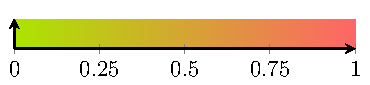
\includegraphics[page=1]{figures/conclusions/figures/main.pdf}
  \\
  \begin{subfigure}{0.48\columnwidth}
    \includegraphics[page=2]{figures/conclusions/figures/main.pdf}
    \caption{2D view}
  \end{subfigure}
  \hfill{}
  \begin{subfigure}{0.48\columnwidth}
    \includegraphics[page=3]{figures/conclusions/figures/main.pdf}
    \caption{3D view}
  \end{subfigure}
  \caption{Likelihood function plot\label{fig:conclusions:likelihood-generalization}}
\end{figure}

Using the above generalization, the probabilities of the two minimal
candidates are calculated as follows:


\begin{equation}
  \begin{split}
    \likelihoodc[\set{1}]{} &=
    \underbrace{ \big((1-c_1) + c_1 \cdot \likelihoodii[\set{1}]{1} \big)}_{t_1}\\
    &\times \underbrace{\big((1 - c_2) + c_2 \cdot \likelihoodii[\set{1}]{2}\big)}_{t_2}\\
    &=\underbrace{\big((1-1) + 1 \cdot (1 - g_1)\big)}_{t_1}\\
    &\times \underbrace{\big((1 - 0.5) + 0.5 \cdot g_1\big)}_{t_2}\\
    &=(1 - g_1) \times (0.5 + 0.5 \cdot g_2)
  \end{split}
\end{equation}

\begin{equation}
  \begin{split}
    \likelihoodc[\set{2}]{} &=
    \underbrace{\big((1-c_1) + c_1 \cdot \likelihoodii[\set{2}]{1}\big)}_{t_1}\\
    &\times \underbrace{\big((1 - c_3) + c_3 \cdot \likelihoodii[\set{2}]{3}\big)}_{t_3}\\
    &=\underbrace{\big((1-1) + 1 \cdot (1 - g_2)\big)}_{t_1}\\
    &\times \underbrace{\big((1 - 1) + 1\cdot g_2\big)}_{t_3}\\
    &=(1 - g_2) \times g_2
  \end{split}
\end{equation}

By performing a \ac{MLE} for both functions it follows that
$\likelihoodc[\set{1}]$ is maximized for $g_1=0$ and
$\likelihood[\set{2}]$ for $g_2 = 0.5$ (\Cref{fig:conclusions:likelihood-plots}).
%
Applying the maximizing values to both expressions, it follows that
$\posteriorc[\set{1}] = 5\e{-4}$ and
$\posteriorc[\set{2}] = 2.5\e{-4}$, entailing the ranking
$\angledlist{\set{1}, \set{2}}$.



\begin{figure}[!ht]
  \begin{subfigure}{0.45\columnwidth}
    \includegraphics[page=4]{figures/conclusions/figures/main.pdf}
    \caption{$\likelihoodc[\set{1}]$}
  \end{subfigure}
  %
  \begin{subfigure}{0.45\columnwidth}
    \includegraphics[page=5]{figures/conclusions/figures/main.pdf}
    \caption{$\likelihoodc[\set{2}]$}
  \end{subfigure}

  \caption{Likelihood plots \label{fig:conclusions:likelihood-plots}}
\end{figure}


Since this generalization is conjectural, future work in this scope
would include evaluating the improvements (if any) introduced by this
generalization.
%
Furthermore, and assuming that this approach yields positive results,
research should done towards automating the process of estimating the
oracles' confidence.
